%%%%%%%%%%%%%%%%%%%% book.tex %%%%%%%%%%%%%%%%%%%%%%%%%%%%%
%
% sample root file for the chapters of your "monograph"
%
% Use this file as a template for your own input.
%
%%%%%%%%%%%%%%%% Springer-Verlag %%%%%%%%%%%%%%%%%%%%%%%%%%


% RECOMMENDED %%%%%%%%%%%%%%%%%%%%%%%%%%%%%%%%%%%%%%%%%%%%%%%%%%%
\documentclass[graybox,envcountchap,sectrefs]{svmono}

% choose options for [] as required from the list
% in the Reference Guide

\usepackage{color}   %May be necessary if you want to color links
\usepackage{hyperref}
\hypersetup{
    colorlinks=false, %set true if you want colored links
    linktoc=all,     %set to all if you want both sections and subsections linked
    linkcolor=red,  %choose some color if you want links to stand out
    urlcolor=blue,
    citecolor=green,
}
\usepackage{mathptmx}
\usepackage{helvet}
\usepackage{courier}
%
\usepackage{type1cm}         

\usepackage{makeidx}         % allows index generation
\usepackage{graphicx}        % standard LaTeX graphics tool
                             % when including figure files
\usepackage{multicol}        % used for the two-column index
\usepackage[bottom]{footmisc}% places footnotes at page bottom

\usepackage{newtxtext}       % 
\usepackage[varvw]{newtxmath}       % selects Times Roman as basic font

% see the list of further useful packages
% in the Reference Guide

\makeindex            % used for the subject index
                       % please use the style svind.ist with
                       % your makeindex program

%%%%%%%%%%%%%%%%%%%%%%%%%%%%%%%%%%%%%%%%%%%%%%%%%%%%%%%%%%%%%%%%%%%%%

\begin{document}


\title{\center{Principles of Mathematical Analysis} \\ \center{THIRD EDITION}}
\author{\center{WALTER RUDIN} \\ \center{Professor of Mathematics} \\ \center{University of Wisconsin-Madison}}
\subtitle{\center{\TeX\;typesetting by Ali Darijani}}

\maketitle

\frontmatter%%%%%%%%%%%%%%%%%%%%%%%%%%%%%%%%%%%%%%%%%%%%%%%%%%%%%%




\tableofcontents
%%%%%%%%%%%%%%%%%%%%%%%foreword.tex%%%%%%%%%%%%%%%%%%%%%%%%%%%%%%%%%
% sample foreword
%
% Use this file as a template for your own input.
%
%%%%%%%%%%%%%%%%%%%%%%%% Springer %%%%%%%%%%%%%%%%%%%%%%%%%%
\Extrachap{Foreward}
%% Please have the foreword written here
Surely, Antoni Zygmund's \textit{Trigonometric Series} has been, and continues to be, one of the most influential 
books in the history of mathematical analysis.Therefore, the current printing, which ensures the future availability of 
this work to the mathematical public is an event of major importance. Its tremendous longevity is a testimony 
to its depth and clarity. Generations of mathematicians from Hardy and Littlewood to recent classes of graduate 
students specializing in analysis have viewed \textit{Trigonometric Series} with enormous admiration and have 
profited greatly from reading it. In light of the importance of Antoni Zygmund as a mathematician and of the 
impact of \textit{Trigonometric Series}, it is only fitting that a brief discussion of his life and mathematics accompany 
the present volume, and this is what I have attempted to give here\footnote[1]{I have been fortunate to have a number of 
excelent references to consult regarding the life of Antoni Zygmund. The reader interested in aditional material 
may consult the references in the bibliography to this Foreword.}. I can only hope that it provides at least 
a small glimpse into the story of this masterpiece and of the man who produced it.\\
\indent Antoni Zygmund was born on December 26, 1900 in Warsaw, Poland. His parents had received relatively 
little education, and were of modest means, so his background was far less privileged than that of the vast majority 
of his colleagues. Zygmund attended school through the middle of high school in Warsaw. When World War I broke 
out, his family was evacuated to Poltava in the Ukraine, where he continued his studies. When the war ended 
in 1918, his family returned to Warsaw, where he completed pre collegiate work, and entered Warsaw University. 
Zygmund's main interest throughout his childhood was astronomy, but at Warsaw University at that time there 
were not sufficient courses offered in that subject to make it realistic as a specialization, and so 
Zygmund turned instead toward another of his interests, mathematics.\\
\indent  There were a number of excelent mathematicians and teachers who profoundly influenced Zygmund during 
this period. The greatest impact came from Aleksander Rajchman and Stanislaw Saks. Rajchman was a junior 
faculty member who was an expert on Riemann's theory of trigonometric series, and Saks a felow student 
who was a few years his senior. From Rajchman, he learned much of the Riemann theory, and his doctoral thesis 
in 1923 was on this subject. Zygmund became an active colaborator with both Rajchman and Saks, publishing 
a number of important articles with each of them. In adition, Saks and Zygmund produced \textit{Analytic Functions}, 
one of the classic texts on complex analysis.\\
\indent One year prior to his PhD, Zygmund was appointed to an instructorship at the Warsaw Polytechnical 
School, and, in 1926, he was appointed Privatdozent at the University of Warsaw. He was awarded a Rockefeller fellowship, 
which he used to travel to England for the academic year of 1929-30 and visit G.H. Hardy at Cambridge 
for the first half of the year, and J.E. Litlewod at Oxford for the second half. This experience had a tremendous 
impact on the young Zygmund. Not only did he work with two of the greatest analysts of the time, but while in 
England, he also met another young mathematician, R.E.A.C. Paley, a student of Littlewod, with whom he had 
an extended and very fruitful collaboration. When he returned to Poland in 1930, Zygmund moved to Wilno where 
he took a chair in mathematics at the Stefan Batory University. It was here that Zygmund's talent and quiet charismasa 
as a teacher of advanced mathematics began to have a very major impact on the field. In the fall of 1930, 
Zygmund met a new student at the University, Jozef Marcinkiewicz. Marcinkiewicz was recognized, even when he 
was a student, as being tremendously talented, with the potential to become a serious mathematician. In the 
following year, which was only the second at Stefan Batory for both teacher and student, Zygmund decided to 
offer a course on trigonometric series preceded by lectures on Lebesgue integration. Marcinkiewicz attended 
this course, and thus began his association with Zygmund. It took just three years for Marcinkiewicz to obtain 
his masters degree, with a thesis that contained the highly non-trivial result that it is possible for 
a continuous periodic function to have interpolating polynomials corresponding to equidistant nodal points 
diverging almost everywhere. This result was elaborated to form his PhD thesis in 1935, and in 1937 Marcinkicwicz 
became Dozent in Wilno. In the period from 1935 to 1939, a collaboration between Marcinkiewicz and Zygmund 
developed that was incredibly successful. Though of relatively short duration, their work opened a number of 
new directions, and in a sense set the stage for the theory of singular integrals which would be Antoni Zygmund's 
greatest contribution.\\
\indent The years in which Zygmund was a young profesor in Wilno, though very productive mathematically, 
were not easy ones. This was due in large part to Zygmund's courageous opposition to the bigotry which was 
all to common around him, and which was supported by the higher authorities. An example of this was his 
strong dislike of anti-Semitic policies with in his university. At one time,for instance, student organizations, 
somewhat analogous to modern day fraternities, were sufficiently influential to mandate that all Jewish 
students must sit on the left side of each classroom during lectures. For Zygmund, this was completely unacceptable 
and in response, he decided to move his classes from the larger hals to small mathematics department seminar rooms 
where there were only long tables in a central arrangement, and hence no seats at the left or right of the 
room. Another illustration of Zygmund's sensitivity to issues of social justice had to do with is university's 
requirement that all student associations have faculty members as their academic sponsors. Zygmund 
regularly sponsored associations which were not in favor with the Polish government. These unpopular moves on 
Zygmund's part did not go unnoticed, and in the year 1931, as part of the political purges of the universities by 
the government, Zygmund was dismissed from his professorship. This immediately brought extremely strong reaction 
from some of the most distinguished mathematicians in Europe.From Lebesgue in France, and  from Hardy and 
Littlewod in England came formal written protests which resulted in Zygmund's reinstatement as professor. 
It is therefore an important aspect of Zygmund's life that, in a very real sense, he was a crusader for human 
rights well before this was fashionable.\\
\indent Among the many remarkable contributions of the Wilno period is the writing of the first version of 
this book, published in Warsaw under the title \textit{Trigonometrical Series}. This was Zygmund's first book, 
and it was published as volume \romannumeral 14 of the series Monografie Matematyczne. This is the same series in which the 
celebrated book \textit{Theorie des Operations Lineaires} by S. Banach appears as volume .The tremendous success 
of \textit{Trigonometrical Series} led to its expansion and revision in to a second edition, published in 1959 
by Cambridge University Press, and then to no fewer than six reprinted versions after that.\\
\indent The time in Wilno which featured the rapid achievement of success came to a sudden end in September 1939 
as World War 2 erupted. At that time, both Zygmund and Marcinkicwicz were mobilized as reserve oficers in 
the Polish army, and, as a result of the temporary ``friendship" between Germany and Russia, Poland was partitioned. 
The Soviets were given control of much of the country, including the part containing Wilno, and they preceded to round up 
and execute many of the Polish officer corps in the Katyn Forest massacre. Most likely, this is how Marcinkiewicz 
perished. Almost by a miracle, Zygmund was able to return to his family and escape with them to the United States, 
but his loss was absolutely devastating. His principal collaborators up to that time besides Marcinkicwicz had 
been Saks, Rajchmanand, Paley. Both Saks and Rajchman were murdered by the Nazis, and Paley had died in a 
tragic accident in 1933. These loses were not just mathematical. Zygmund had been extremely close to each of 
them, and so the war period must surely have been one of the most difficult of his life.\\
\indent By 1939, Zygmund had an international reputation, and many friends all over the mathematical world. It was due 
to the efforts of some of these friends, such as Jacob Tamarkin, Jerzy Neyman and Norbert Wiener, that Zygmund was 
able to emigrate to the United States in 1940. During the time immediately prior to the United States entering 
in to the war, there were very few jobs available to mathematicians. Nevertheless, after teaching for a 
semester at MIT, Zygmund was offered and accepted a position at Mount Holyoke College in central Massachusetts. 
A few years later, other offers followed. In 1945, Zygmund became a professor at the University of Pennsylvania, 
and then, in 1947, he was offered a professorship at the University of Chicago.\\
\indent The University of Chicago mathematics department, which had had a tradition of great strength, 
had experienced a period of decline prior to World War 2. During the war, the president of the university, 
Robert Maynard Hutchins, brought the Manhatan project to the campus, and with it camea number of outstanding 
scientists, such as Enrico Fermi. Hutchins then decided to make it a priority to strengthen the mathematics 
department in order to match the high quality of physical science apointments that had been made. To this end, 
a new chairman, Marshal Stone, was brought to the university and asked to bring about this improvement. 
The result was some thing phenomenal. In the period just after the war, Stone was able to asemble one of the 
best mathematics departments in history. At this time, the faculty of mathematics included such members as A.A. Albert, 
S.S. Chern, L. Graves, P. Halmos, I. Kaplansky, S. MacLane, I. Segal, E. Spanier, M. Stone, A. Weil and A. Zygmund. 
Together with this influx of great mathematicians there came a corresponding influx of brilliant students.\\
\indent The combination of such a strong mathematician and teacher as Zygmund with the unusualy rich mathematical 
environment of the University of Chicago produced a golden period of creativity and of supervision of exceptional 
students for Zygmund that was the crowning achievement of his life's work. In several cases, the route of 
outstanding students to Chicago was not totally straightforward, and the most famous case was that of Alberto P. Calderon. 
The story of the means by which Calderon came to Chicago is legendary. The following, taken from the introduction 
to the book, \textit{Essays in Honor of Alberto P.Calderon}~\cite{albertohonor} tells the story beautifuly:\\
\noindent In the years imediately after World War 2, the U.S. Department of State had a very active visitors 
program that sent prominent scientists to Latin America. Thus, Adrian Albert, Marshal Stone, and George Birkhoff 
visited Buenos Aires, and Gonzalez Dominguez arranged through them the visit of Zygmund, whose work on Fourier Series 
he much admired. At the Institute of Mathematics, Zygmund gave a two-month seminar on topics in analysis, 
based on his book. This seminar was atended by Gonzalez Dominguez, Calderon, Mischa Cotlar, and three other 
young Argentine mathematicians. Each of the participants had to discus a portion of the text. Calderon's 
assignment was to present the Marcel Riesz theorem on the continuity of the Hilbert transform in $L^p$. 
According to Cotlar's vivid recollection of the event, Calderon's exposition was entirely aceptable to the 
junior audience, but not to Zygmuncl, who appeared agitated and grimaced all the time. Finally, he interrupted 
Calderon abruptly to ask where had read the material he was presenting, and a bewildered Calderon answered 
that he had read it in Zygmund's book. Zygmund vehemently informed the audience that this was not the proof 
in his book, and after the lecture took Calderon aside and quized him about the new short and elegant proof. 
Calderon confessed that he had first tried to prove the theorem by himself, and then thinking he could not 
do it, had read the begining of the proof in the book; but after the first couple of lines, instead of turning 
the page, had figured out how the proof would finish. In fact, he had found himself an elegant new proof of 
the Riesz Theorem! Zygmund imediately recognized Calderon's power and then and there decided to invite him to 
Chicago to study wit him.\\
\indent This anecdote illustrates one of Calderon's main characteristics\dots \\ \\
\noindent The anecdote above also illustrates one of Zygmund's main characteristics: His tremendous desire to 
work with people of the greatest mathematic ability, and his absolute devotion to those people. Calderon 
came to the University of Chicago in 1949 on a Rockefeller fellowship, and only one year later received his 
PhD there under Zygmund's supervision. The thesis consisted of three research papers, each of which was a major 
work. In particular, among the results of the thesis was one of the greatest importance, concerning the boundary 
behavior of harmonic functions of several variables, which represented a crucial step in carying out the real 
variable program of Zygmund which will be described below. The collaboration betwen Calderon and Zygmund which 
followed was certainly one of the greatest in the history of modern analysis, and created a theory, the so-called 
Calderon-Zygmund Theory of Singular Integrals, that not only allowed for the extension of much of classical 
Fourier analysis from one to several dimensions,but played a fundamental role in the development of the theories 
of partial differential equations and geometry as well.\\
\indent More than simply creating a new powerful mathematical theory at Chicago, Zygmund created a school, 
the Chicago School of Analysis, which was to have an enormous impact on the subject in the next five decades, 
and promises to continue to do so in the future. After Calderon, there came other students who worked with 
Zygmund and who individually made historic contributions to mathematics. In 1955, Elias M. Stein received his 
doctorate under Zygmund, and, as is well known, by his brilliant research and teaching went on to establish 
a great school at Princeton. A bit later, other remarkable students finished their thesis work with Zygmund, 
including Paul Cohen and Guido and Mary Weiss. Taking into account the generations of students whose mathematical 
ancestry is traceable back to Zygmund, it is hard to imagine what mathematical analysis would be like without 
their collective contribution.\\
\indent At Chicago, Zygmund had a total of thirty-five students. His collected works include some 215 articles. 
Zygmund received many formal honors in his lifetime. He was a recipient of the Steele Prize of the American 
Mathematical Society, as well as the National Medal of Science, the highest award given by the United States 
government in recognition of scientific achievement. In addition, he was given membership of a number of academics, 
including the National Academy of Sciences and the American Academy for Arts and Sciences(USA), the Polish 
Academy of Sciences, the Argentina Academy of Sciences, Royal Academy of Sciences of Spain, and the Academy, 
of Arts and Sciences of Palermo, Italy. Zygmund also held honorary degrees from Washington University, the 
University of Torun, Poland, the University of Paris and the University of Uppsala, Sweden.\\
\indent After a very long and productive life in which he published his last, research article at the age of 
79, he finally slowed considerably, and, after a long illness, died at the age of 91. Few mathematicians have 
provided such a striking and wonderful counter example to G.H. Hardy's view on the rapidity of loss of creativity 
that mathematicians suffer with age.\\
\indent Zygmund's life events and his mathematics, particularly that covered in the present volume, are heavily 
intertwined. In what follows, I would like to discuss this mathematics in the context of the historical perspective 
considered above.\\
\indent continued:-)






\vspace{\baselineskip}
\begin{flushright}\noindent
University of Chicago, \hfill {\it Robert A. Fefferman}\\
\end{flushright}



%%%%%%%%%%%%%%%%%%%%%%preface.tex%%%%%%%%%%%%%%%%%%%%%%%%%%%%%%%%%%%%%%%%%
% sample preface
%
% Use this file as a template for your own input.
%
%%%%%%%%%%%%%%%%%%%%%%%% Springer %%%%%%%%%%%%%%%%%%%%%%%%%%
\Extrachap{PREFACE}
\preface

%% Please write your preface here

This book is intended to serve as a text for the course in analysis that is usually taken by advanced 
undergraduates or by first-year students who study mathematics.\\
\indent The present edition covers essentially the same topics as the second one,
with some additions, a few minor omissions, and considerable rearrangement. I hope that these changes will 
make the material more accessible and more attractive to the students who take such a course.\\
\indent Experience has convinced me that it is pedagogically unsound (though logically correct) to start off 
with the construction of the real numbers from the rational ones. At the beginning, most students simply 
fail to appreciate the need for doing this. Accordingly, the real number system is introduced as an ordered 
field with the least-upper-bound property, and a few interesting applications of this property are quickly made. 
However, Dedekind's construction is not omitted. It is now in an Appendix to Chapter 1, where it may be 
studied and enjoyed whenever the time seems ripe.\\
\indent The material on functions of several variables is almost completely rewritten, with many details filled in, 
and with more examples and more motivation. The proof of the inverse function theorem--the key item in Chapter 9--is
simplified by means of the fixed point theorem about contraction mappings. Differential forms are discussed 
in much greater detail. Several applications of Stokes' theorem are included.\\
\indent As regards other changes, the chapter on the Riemann-Stieltjes integral has been trimmed a bit, a short 
do-it-yourself section on the gamma function has been added to Chapter 8, and there is a large number of new exercises, 
most of them with fairly detailed hints.\\
\indent I have also included several references to articles appearing in the \textit{American Mathe1natical Monthly} 
and in \textit{Mathematics Magazine}, in the hope that students will develop the habit of looking into the 
journal literature. Most of these references were kindly supplied by R. B. Burckel.\\
\indent Over the years, many people, students as well as teachers, have sent me corrections, criticism, and 
other comments concerning the previous editions of this book. I have appreciated these, and I take this 
opportunity to express my sincere thanks to all who have written me.
\vspace{\baselineskip}
\begin{flushright}\noindent
\hfill {\bf WALTER RUDIN}\\
\end{flushright}

%%%%%%%%%%%%%%%%%%%%%%%acknow.tex%%%%%%%%%%%%%%%%%%%%%%%%%%%%%%%%%%%%%%%%%
% sample acknowledgement chapter
%
% Use this file as a template for your own input.
%
%%%%%%%%%%%%%%%%%%%%%%%% Springer %%%%%%%%%%%%%%%%%%%%%%%%%%

\Extrachap{Acknowledgements}

Use the template \emph{acknow.tex} together with the document class SVMono (monograph-type books) or SVMult (edited books) if you prefer to set your acknowledgement section as a separate chapter instead of including it as last part of your preface.

I would like to thank my 



%%%%%%%%%%%%%%%%%%%%%%% dedic.tex %%%%%%%%%%%%%%%%%%%%%%%%%%%%%%%%%
%
% sample dedication
%
% Use this file as a template for your own input.
%
%%%%%%%%%%%%%%%%%%%%%%%% Springer %%%%%%%%%%%%%%%%%%%%%%%%%%
%\extrachap{Dedication}
\begin{dedication}
\center{DEDICATED TO THE MEMORIES OF}\\
\center{A. RAJCHMAN AND J. MARCINKIEWIC}\\
\center{MY TEACHER AND MY PUPIL}\\
\end{dedication}








\mainmatter%%%%%%%%%%%%%%%%%%%%%%%%%%%%%%%%%%%%%%%%%%%%%%%%%%%%%%%
%%%%%%%%%%%%%%%%%%%%%%part.tex%%%%%%%%%%%%%%%%%%%%%%%%%%%%%%%%%%
% 
% sample part title
%
% Use this file as a template for your own input.
%
%%%%%%%%%%%%%%%%%%%%%%%% Springer %%%%%%%%%%%%%%%%%%%%%%%%%%

\begin{partbacktext}
\part{(VOLUME I)}

\end{partbacktext}

%%%%%%%%%%%%%%%%%%%%% chapter.tex %%%%%%%%%%%%%%%%%%%%%%%%%%%%%%%%%
%
% sample chapter
%
% Use this file as a template for your own input.
%
%%%%%%%%%%%%%%%%%%%%%%%% Springer-Verlag %%%%%%%%%%%%%%%%%%%%%%%%%%
%\motto{And Ken Said Let Everything Be A File...And Then There Was Light...}
\chapter{THE REAL AND COMPLEX NUMBER SYSTEMS}
\label{intro} % Always give a unique label
% use \chaptermark{}
% to alter or adjust the chapter heading in the running head


% \abstract{
    % test
% }
\section{\textbf{INTRODUCTION}}
A satisfactory discussion of the main concepts of analysis (such as convergence, continuity, differentiation, and integration) 
must be based on an accurately defined number concept. We shall not, however, enter into any discussion of 
the axioms that govern the arithmetic of the integers, but assume familiarity with the rational numbers 
(i.e., the numbers of the form $\frac{m}{n}$, where $m$ and $n$ are integers and $n\not=0$).\\
The rational number system is inadequate for many purposes, both as a field and as an ordered set. (These terms will 
be defined in Secs. ~\ref{to be added} and ~\ref{to be added}.) For instance, there is no rational $p$ such that 
$p^2=2$. (We shall prove this presently.) This leads to the introduction of so-called ``irrational numbers'' 
which are often written as infinite decimal expansions and are considered to be ``approximated'' by the corresponding 
finite decimals. Thus the sequence
\begin{equation*}
    1, 1.4, 1.41, 1.414, 1.4142, \dots
\end{equation*}
``tends to $\sqrt{2}$.'' But unless the irrational number $\sqrt{2}$ has been clearly defined, the question must arise: 
Just what is it that this sequence ``tends to''?\\
\indent This sort of question can be answered as soon as the so-called ``real number system'' is constructed.

\subsection*{\textbf{Example}}
\label{subsec:1}
We now show that the equation
\begin{equation}
    \label{eq:01}
    p^2=2
\end{equation}
is not satisfied by any rational $p$. If there were such a $p$, we could write $p=\frac{m}{n}$ where $m$ and $n$ 
are integers that are not both even. Let us assume this is done. Then ~\ref{eq:01} implies
\begin{equation}
    \label{eq:02}
    m^2=2n^2,
\end{equation}
This shows that $m^2$ is even. Hence $m$ is even (if $m$ were odd, $m^2$ would be odd), and so $m^2$ is divisible by $4$.
It follows that the right side of ~\ref{eq:02} is divisible by $4$, so that $n^2$ is even, which implies that $n$ 
is even.\\
\indent The assumption that ~\ref{eq:01} holds thus leads to the conclusion that both $m$ and $n$ are even, contrary 
to our choice of $m$ and $n$. Hence ~\ref{eq:01} is impossible for the rational $p$.\\
\indent We now examine this situation a little more closely. Let $\mathbf{A}$ be the set of all positive rationals $p$ such that $p^2 < 2$ 
and let $B$ consist of all positive rationals $p$ such that $^2 > 2$. We shall show that $\mathbf{A}$ \textit{contains no largest number and}
 $\mathbf{B}$ \textit{contains no smallest}.\\
 \indent More explicitly, for every $p$ in $\mathbf{A}$ we can find a rational $p$ in $\mathbf{A}$ such that 
 $p<q$, and for every $p$ in $\mathbb{B}$ we can find a rational $q$ in $\mathbf{B}$ such that $q<p$.\\
 \indent To do this, we associate with each rational $p>0$ the number
 \begin{equation}
    \label{eq:03}
    q=p-\frac{p^2-2}{p+2}=\frac{2p+2}{p+2}
 \end{equation}
\noindent Then
\begin{equation}
    \label{eq:04}
    q^2-2=\frac{2(p^2-2)}{(p+2)^2}
\end{equation}
\indent If $p$ is in $\mathbf{A}$ then $p^2-2<0$, ~\ref{eq:03} shows that $q>p$, and ~\ref{eq:04} shows that
$q^2<2$. Thus $q$ is in $\mathbf{A}$.\\
\indent If $p$ is in $\mathbf{B}$ then $p^2-2>0$, ~\ref{eq:03} shows that $0<q<p$, and ~\ref{eq:04} shows that
$q^2>2$. Thus $q$ is in $\mathbf{B}$.

\subsection*{\textbf{Remark}}
The purpose of the above discussion has been to show that the rational number system has certain gaps, in spite 
of the fact that between any two rational there is another: If $r<s$ then $r<(r+s)/2<s$. The real number system
fills these gaps. This is the principal reason for the fundamental role which it plays in analysis.\\
\indent In order to elucidate its structure, as well as that of the complex numbers, we start with a brief
 discussion of the general concepts of the \textit{ordered set} and \textit{field}.\\
 \indent Here is some of the standard set-theoretic terminology that will be used throughout this book.

 \begin{definition}
    If $\mathbf{A}$ is any set (whose elements may be numbers or any other objects), we write $x \in \mathbf{A}$
    to indicate that $x$ is a member (or an element) of $\mathbf{A}$.\\
    \indent If $x$ is not a member of $\mathbf{A}$, we write: $x \notin \mathbf{A}$\\
    \indent The set which contains no element will be called the \textit{empty set}. If a set has at least 
    one element, it is called \textit{nonempty}.\\
    \indent If $\mathbf{A}$ and $\mathbf{B}$ are sets, and if every element if $\mathbf{A}$ is an element of $\mathbf{B}$,
    we say that $\mathbf{A}$ is a subset of $\mathbf{B}$, and write $\mathbf{A} \subset \mathbf{B}$, or 
    $\mathbf{B} \supset \mathbf{A}$. If, in addition, there is an element of $\mathbf{B}$ which is not in 
    $\mathbf{A}$, then $\mathbf{A}$ is said to b a \textit{proper } subset of $\mathbf{B}$. Note 
    that $\mathbf{A} \subset \mathbf{A}$ for every set $\mathbf{A}$.
    \indent If $\mathbf{A} \subset \mathbf{B}$ and $\mathbf{B} \subset \mathbf{A}$ , we write $\mathbf{A}=\mathbb{B}$. Otherwise 
    $\mathbf{A} \neq \mathbf{B}$.
\end{definition}

\begin{definition}
    throughout this chapter, the set of all rational numbers will be denoted by $\mathit{Q}$.
\end{definition}

\section*{\textbf{ORDERED SETS}}

\begin{definition}
    Let $\mathit{S}$ be a set. An \textit{order} on $\mathit{S}$ is a relation, denoted by $<$, with 
    the following two properties:
    \begin{itemize}
        \item If $x \in \mathit{S}$ and $y \in \mathit{S}$ then one and only one the statements
    \begin{equation*}
        x<y,\quad x=y,\quad y<x
    \end{equation*}
    is true.
    \item If $x,y,z \in \mathit{S}$, if $x<y$ and $y<x$, then $x<z$.
    The statement ``$x<y$'' may be read as ``$x$ is less than $y$'' or ``$x$ is smaller than $y$'' 
    or ``$x$ precedes $y$''.\\
    It is often convenient to write $y>x$ in place of $x<y$.\\
    The notation $x \leq y$ indicates that $x<y$ or $x=y$, without specifying which of these two is to hold. 
    In other words, $x \leq y$ is the negation of $x>y$.
    \end{itemize}
\end{definition}

\begin{definition}
    An \textit{ordered set} is set $\mathit{S}$ in which an order is defined.\\
    For example, $\mathit{Q}$ is an ordered set if $r<s$ is defined to mean that $r-s$ is a positive rational number.
\end{definition}




\begin{definition}
    A field is a set $F$ with two operations, called \textit{addition} and \textit{multiplication},
    which satisfy the following so-called ``field axioms'' ~\ref{AXIOMSA}, and ~\ref{AXIOMSM}, and ~\ref{AXIOMSD}:


\subsubsection*{\textbf{Axioms for addition}}
\label{AXIOMSA}
\begin{itemize}
    \item If $x \in F$ and $y \in F$, then their sum $x+y$ is in $F$.
    \item Addition is commutative: $x+y=y+x$ for all $x,y \in F$
    \item Addition is associative: $(x+y)+z=x+(y+z)$ for all $x,y,z \in F$.
    \item $F$ contains an element $0$ such that $0+x=x$ for every $x \in F$.
    \item To every $x \in F$ corresponds an element $-x \in F$ such That
        \begin{equation*}
            x+(-x)=0.
        \end{equation*} 
\end{itemize}
\subsubsection*{\textbf{Axioms for multiplication}}
\label{AXIOMSM}
\begin{itemize}
    \item If $x \in F$ and $y \in F$, then their product $xy$ is in $F$.
    \item Multiplication is commutative: $xy=yx$ for all $x,y \in F$.
    \item Multiplication is associative: $(xy)z=x(yz)$ for all $x,y,z \in F$.
    \item $F$ contains an element $1 \neq 0$ such that $1x=x$ for every $x \in F$.
    \item If $x \in F$ and $x \neq 0$ then there exists an element $1/x \in F$ such that
    \begin{equation*}
        x.(1/x)=1.
    \end{equation*}
\end{itemize}

\subsubsection*{\textbf{The distributive law}}
\label{AXIOMSD}

\begin{equation*}
    x(y+z)=xy+xz
\end{equation*}
holds for all $x,y,z \in F$.
\end{definition}


\begin{theorem}
Theorem IS BEST USED LIKE THIS
\end{theorem}

\subsection*{\textbf{Remark}}
\label{sec:2}

\subsection*{\textbf{Definition}}
\label{sec:3}

\subsection*{\textbf{Definition}}
\label{sec:4}

\section{ORDERED SETS}







\subsection*{\textbf{Example}}
\label{sec:5}
\subsection*{\textbf{Example}}
\label{sec:6}
\subsection*{\textbf{Example}}
\label{sec:7}
\subsection*{\textbf{Example}}
\label{sec:8}
\subsection*{\textbf{Example}}
\label{sec:9}
\subsection*{\textbf{Example}}
\label{sec:10}
\subsection*{\textbf{Example}}
\label{sec:11}


\section{FIELDS}

\subsection*{\textbf{Example}}
\label{sec:12}


\subsection*{\textbf{Example}}
\label{sec:14}
\subsection*{\textbf{Example}}
\label{sec:15}
\subsection*{\textbf{Example}}
\label{sec:16}
\subsection*{\textbf{Example}}
\label{sec:17}
\subsection*{\textbf{Example}}
\label{sec:18}


\section{THE REAL FIELD}

\subsection*{\textbf{Example}}
\label{sec:19}
\label{sec:22}


\section*{THE EXTENDED REAL NUMBER SYSTEM}
\subsection*{\textbf{Example}}
\label{sec:23}



\section{THE COMPLEX FIELD}

\subsection*{\textbf{Example}}
\label{sec:24}

\subsection*{\textbf{Example}}
\label{sec:25}


\subsection*{\textbf{Example}}
\label{sec:26}

\subsection*{\textbf{Example}}
\label{sec:27}
\subsection*{\textbf{Example}}
\label{sec:28}
\subsection*{\textbf{Example}}
\label{sec:29}
\subsection*{\textbf{Example}}
\label{sec:30}
\subsection*{\textbf{Example}}
\label{sec:31}
\subsection*{\textbf{Example}}
\label{sec:32}
\subsection*{\textbf{Example}}
\label{sec:33}
\subsection*{\textbf{Example}}
\label{sec:34}
\subsection*{\textbf{Example}}
\label{sec:35}

\section{EUCLIDEAN SPACES}
\subsection*{\textbf{Example}}
\label{sec:36}

\subsection*{\textbf{Example}}
\label{sec:37}
\subsection*{\textbf{Example}}
\label{sec:38}

\section{APPENDIX}

\subsection*{\textbf{Step}}
\label{sec:37}












\label{sec:0}
\begin{programcode}{basic usage}
\begin{verbatim}
brew install
    fgjn
\end{verbatim}
\end{programcode}



\section{Section Heading}
\label{sec:1}
Use the template \emph{chapter.tex} together with the document class SVMono (monograph-type books) or SVMult (edited books) to style the various elements of your chapter content conformable to the Springer Nature layout.

\section{Section Heading}
\label{sec:2}
% Always give a unique label
% and use \ref{<label>} for cross-references
% and \cite{<label>} for bibliographic references
% use \sectionmark{}
% to alter or adjust the section heading in the running head
Instead of simply listing headings of different levels we recommend to let every heading be followed by at least a short passage of text. Furtheron please use the \LaTeX\ automatism for all your cross-references and citations.

Please note that the first line of text that follows a heading is not indented, whereas the first lines of all subsequent paragraphs are.

\eject

Use the standard \verb|equation| environment to typeset your equations, e.g.
%
\begin{equation}
a \times b = c\;,
\end{equation}
%
however, for multiline equations we recommend to use the \verb|eqnarray| environment\footnote{In physics texts please activate the class option \texttt{vecphys} to depict your vectors in \textbf{\itshape boldface-italic} type - as is customary for a wide range of physical subjects.}.
\begin{eqnarray}
\left|\nabla U_{\alpha}^{\mu}(y)\right| &\le&\frac1{d-\alpha}\int
\left|\nabla\frac1{|\xi-y|^{d-\alpha}}\right|\,d\mu(\xi) =
\int \frac1{|\xi-y|^{d-\alpha+1}} \,d\mu(\xi)\qquad  \\
&=&(d-\alpha+1) \int\limits_{d(y)}^\infty
\frac{\mu(B(y,r))}{r^{d-\alpha+2}}\,dr \le (d-\alpha+1)
\int\limits_{d(y)}^\infty \frac{r^{d-\alpha}}{r^{d-\alpha+2}}\,dr
\label{eq:10}
\end{eqnarray}

\enlargethispage{24pt}

\subsection{Subsection Heading}
\label{subsec:2}
Instead of simply listing headings of different levels we recommend to let every heading be followed by at least a short passage of text. Further on please use the \LaTeX\ automatism for all your cross-references\index{cross-references} and citations\index{citations} as has already been described in Sect.~\ref{sec:2}.

\begin{quotation}
Please do not use quotation marks when quoting texts! Simply use the \verb|quotation| environment -- it will automatically be rendered in the preferred layout.
\end{quotation}


\subsubsection{Subsubsection Heading}
Instead of simply listing headings of different levels we recommend to let every heading be followed by at least a short passage of text. Furtheron please use the \LaTeX\ automatism for all your cross-references and citations as has already been described in Sect.~\ref{subsec:2}, see also Fig.~\ref{fig:1}\footnote{If you copy text passages, figures, or tables from other works, you must obtain \textit{permission} from the copyright holder (usually the original publisher). Please enclose the signed permission with the manucript. The sources\index{permission to print} must be acknowledged either in the captions, as footnotes or in a separate section of the book.}

Please note that the first line of text that follows a heading is not indented, whereas the first lines of all subsequent paragraphs are.

% For figures use
%
\begin{figure}[b]
\sidecaption
% Use the relevant command for your figure-insertion program
% to insert the figure file.
% For example, with the option graphics use
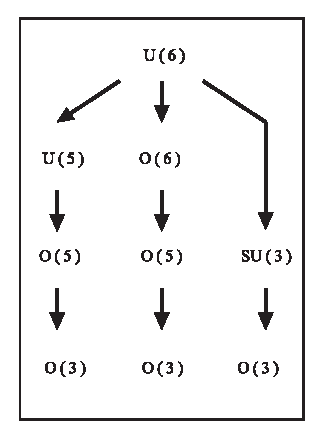
\includegraphics[scale=.65]{figure}
%
% If not, use
%\picplace{5cm}{2cm} % Give the correct figure height and width in cm
%
\caption{If the width of the figure is less than 7.8 cm use the \texttt{sidecapion} command to flush the caption on the left side of the page. If the figure is positioned at the top of the page, align the sidecaption with the top of the figure -- to achieve this you simply need to use the optional argument \texttt{[t]} with the \texttt{sidecaption} command}
\label{fig:1}       % Give a unique label
\end{figure}


\paragraph{Paragraph Heading} %
Instead of simply listing headings of different levels we recommend to let every heading be followed by at least a short passage of text. Furtheron please use the \LaTeX\ automatism for all your cross-references and citations as has already been described in Sect.~\ref{sec:2}.

Please note that the first line of text that follows a heading is not indented, whereas the first lines of all subsequent paragraphs are.

For typesetting numbered lists we recommend to use the \verb|enumerate| environment -- it will automatically render Springer's preferred layout.

\begin{enumerate}
\item{Livelihood and survival mobility are oftentimes coutcomes of uneven socioeconomic development.}
\begin{enumerate}
\item{Livelihood and survival mobility are oftentimes coutcomes of uneven socioeconomic development.}
\item{Livelihood and survival mobility are oftentimes coutcomes of uneven socioeconomic development.}
\end{enumerate}
\item{Livelihood and survival mobility are oftentimes coutcomes of uneven socioeconomic development.}
\end{enumerate}


\subparagraph{Subparagraph Heading} In order to avoid simply listing headings of different levels we recommend to let every heading be followed by at least a short passage of text. Use the \LaTeX\ automatism for all your cross-references and citations as has already been described in Sect.~\ref{sec:2}, see also Fig.~\ref{fig:2}.

Please note that the first line of text that follows a heading is not indented, whereas the first lines of all subsequent paragraphs are.

For unnumbered list we recommend to use the \verb|itemize| environment -- it will automatically render Springer's preferred layout.

\begin{itemize}
\item{Livelihood and survival mobility are oftentimes coutcomes of uneven socioeconomic development, cf. Table~\ref{tab:1}.}
\begin{itemize}
\item{Livelihood and survival mobility are oftentimes coutcomes of uneven socioeconomic development.}
\item{Livelihood and survival mobility are oftentimes coutcomes of uneven socioeconomic development.}
\end{itemize}
\item{Livelihood and survival mobility are oftentimes coutcomes of uneven socioeconomic development.}
\end{itemize}

\begin{figure}[t]
\sidecaption[t]
% Use the relevant command for your figure-insertion program
% to insert the figure file.
% For example, with the option graphics use
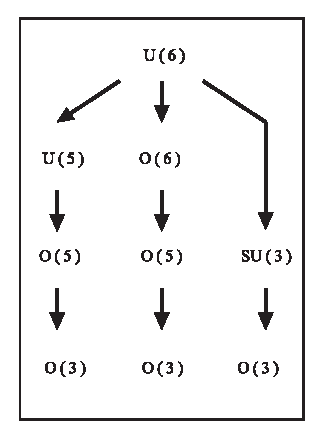
\includegraphics[scale=.65]{figure}
%
% If not, use
%\picplace{5cm}{2cm} % Give the correct figure height and width in cm
%
\caption{Please write your figure caption here}
\label{fig:2}       % Give a unique label
\end{figure}

\runinhead{Run-in Heading Boldface Version} Use the \LaTeX\ automatism for all your cross-references and citations as has already been described in Sect.~\ref{sec:2}.

\subruninhead{Run-in Heading Boldface and Italic Version} Use the \LaTeX\ automatism for all your cross-refer\-ences and citations as has already been described in Sect.~\ref{sec:2}\index{paragraph}.

\subsubruninhead{Run-in Heading Displayed Version} Use the \LaTeX\ automatism for all your cross-refer\-ences and citations as has already been described in Sect.~\ref{sec:2}\index{paragraph}.
% Use the \index{} command to code your index words
%
% For tables use
%
\begin{table}[!t]
\caption{Please write your table caption here}
\label{tab:1}       % Give a unique label
%
% For LaTeX tables use
%
\begin{tabular}{p{2cm}p{2.4cm}p{2cm}p{4.9cm}}
\hline\noalign{\smallskip}
Classes & Subclass & Length & Action Mechanism  \\
\noalign{\smallskip}\svhline\noalign{\smallskip}
Translation & mRNA$^a$  & 22 (19--25) & Translation repression, mRNA cleavage\\
Translation & mRNA cleavage & 21 & mRNA cleavage\\
Translation & mRNA  & 21--22 & mRNA cleavage\\
Translation & mRNA  & 24--26 & Histone and DNA Modification\\
\noalign{\smallskip}\hline\noalign{\smallskip}
\end{tabular}
$^a$ Table foot note (with superscript)
\end{table}
%
\section{Section Heading}
\label{sec:3}
% Always give a unique label
% and use \ref{<label>} for cross-references
% and \cite{<label>} for bibliographic references
% use \sectionmark{}
% to alter or adjust the section heading in the running head
Instead of simply listing headings of different levels we recommend to let every heading be followed by at least a short passage of text. Furtheron please use the \LaTeX\ automatism for all your cross-references and citations as has already been described in Sect.~\ref{sec:2}.

Please note that the first line of text that follows a heading is not indented, whereas the first lines of all subsequent paragraphs are.

If you want to list definitions or the like we recommend to use the Springer-enhanced \verb|description| environment -- it will automatically render Springer's preferred layout.

\begin{description}[Type 1]
\item[Type 1]{That addresses central themes pertainng to migration, health, and disease. In Sect.~\ref{sec:1}, Wilson discusses the role of human migration in infectious disease distributions and patterns.}
\item[Type 2]{That addresses central themes pertainng to migration, health, and disease. In Sect.~\ref{subsec:2}, Wilson discusses the role of human migration in infectious disease distributions and patterns.}
\end{description}

\subsection{Subsection Heading} %
In order to avoid simply listing headings of different levels we recommend to let every heading be followed by at least a short passage of text. Use the \LaTeX\ automatism for all your cross-references and citations citations as has already been described in Sect.~\ref{sec:2}.

Please note that the first line of text that follows a heading is not indented, whereas the first lines of all subsequent paragraphs are.

\begin{svgraybox}
If you want to emphasize complete paragraphs of texts we recommend to use the newly defined Springer class option \verb|graybox| and the newly defined environment \verb|svgraybox|. This will produce a 15 percent screened box 'behind' your text.

If you want to emphasize complete paragraphs of texts we recommend to use the newly defined Springer class option and environment \verb|svgraybox|. This will produce a 15 percent screened box 'behind' your text.
\end{svgraybox}


\subsubsection{Subsubsection Heading}
Instead of simply listing headings of different levels we recommend to let every heading be followed by at least a short passage of text. Furtheron please use the \LaTeX\ automatism for all your cross-references and citations as has already been described in Sect.~\ref{sec:2}.

Please note that the first line of text that follows a heading is not indented, whereas the first lines of all subsequent paragraphs are.

\begin{theorem}
Theorem text goes here.snwkeJFNKwjenfkwjenF
\end{theorem}
%
% or
%
\begin{definition}
Definition text goes here.
\end{definition}

\begin{proof}
%\smartqed
Proof text goes here.
%\qed
\end{proof}

\paragraph{Paragraph Heading} %
Instead of simply listing headings of different levels we recommend to let every heading be followed by at least a short passage of text. Furtheron please use the \LaTeX\ automatism for all your cross-references and citations as has already been described in Sect.~\ref{sec:2}.

Note that the first line of text that follows a heading is not indented, whereas the first lines of all subsequent paragraphs are.
%
% For built-in environments use
%
\begin{theorem}
Theorem text goes here.
\end{theorem}
%
\begin{definition}
Definition text goes here.
\end{definition}
%
\begin{proof}
%\smartqed
Proof text goes here.
%\qed
\end{proof}
%
%
\begin{trailer}{Trailer Head}
If you want to emphasize complete paragraphs of texts in an \verb|Trailer Head| we recommend to
use  \begin{verbatim}\begin{trailer}{Trailer Head}
...
\end{trailer}\end{verbatim}
\end{trailer}
%
\begin{question}{Questions}
If you want to emphasize complete paragraphs of texts in an \verb|Questions| we recommend to
use  \begin{verbatim}\begin{question}{Questions}
...
\end{question}\end{verbatim}
\end{question}
%
%
\begin{important}{Important}
If you want to emphasize complete paragraphs of texts in an \verb|Important| we recommend to
use  \begin{verbatim}\begin{important}{Important}
...
\end{important}\end{verbatim}
\end{important}
%
\clearpage
\begin{warning}{Attention}
If you want to emphasize complete paragraphs of texts in an \verb|Attention| we recommend to
use  \begin{verbatim}\begin{warning}{Attention}
...
\end{warning}\end{verbatim}
\end{warning}

\begin{programcode}{Program Code}
If you want to emphasize complete paragraphs of texts in an \verb|Program Code| we recommend to
use

\verb|\begin{programcode}{Program Code}|

\verb|\begin{verbatim}...\end{verbatim}|

\verb|\end{programcode}|

\end{programcode}
%
\begin{tips}{Tips}
If you want to emphasize complete paragraphs of texts in an \verb|Tips| we recommend to
use  \begin{verbatim}\begin{tips}{Tips}
...
\end{tips}\end{verbatim}
\end{tips}
%
%
\begin{overview}{Overview}
If you want to emphasize complete paragraphs of texts in an \verb|Overview| we recommend to
use  \begin{verbatim}\begin{overview}{Overview}
...
\end{overview}\end{verbatim}
\end{overview}
\clearpage
\begin{backgroundinformation}{Background Information}
If you want to emphasize complete paragraphs of texts in an \verb|Background|
\verb|Information| we recommend to
use

\verb|\begin{backgroundinformation}{Background Information}|

\verb|...|

\verb|\end{backgroundinformation}|
\end{backgroundinformation}
\begin{legaltext}{Legal Text}
If you want to emphasize complete paragraphs of texts in an \verb|Legal Text| we recommend to
use  \begin{verbatim}\begin{legaltext}{Legal Text}
...
\end{legaltext}\end{verbatim}
\end{legaltext}
%
\begin{acknowledgement}
If you want to include acknowledgments of assistance and the like at the end of an individual chapter please use the \verb|acknowledgement| environment -- it will automatically render Springer's preferred layout.
\end{acknowledgement}
%
\section*{Appendix}
\addcontentsline{toc}{section}{Appendix}
%
When placed at the end of a chapter or contribution (as opposed to at the end of the book), the numbering of tables, figures, and equations in the appendix section continues on from that in the main text. Hence please \textit{do not} use the \verb|appendix| command when writing an appendix at the end of your chapter or contribution. If there is only one the appendix is designated ``Appendix'', or ``Appendix 1'', or ``Appendix 2'', etc. if there is more than one.

\begin{equation}
a \times b = c
\end{equation}
% Problems or Exercises should be sorted chapterwise
\section*{Problems}
\addcontentsline{toc}{section}{Problems}
%
% Use the following environment.
% Don't forget to label each problem;
% the label is needed for the solutions' environment
\begin{prob}
\label{prob1}
If $r$ is rational $(r \neq 0)$ and $x$ is irrational, prove that $r+x$ and $rx$ are irrational.
\end{prob}

\begin{prob}
\label{prob2}
If $r$ is rational $(r\neq 0)$ and $x$ is irrational, prove that $r+x$ and $rx$ are irrational.
\end{prob}

\begin{prob}
\label{prob3}
If $r$ is rational $(r\not0)$ and $x$ is irrational, prove that $r+x$ and $rx$ are irrational.
\end{prob}

\begin{prob}
\label{prob4}
If $r$ is rational $(r\not0)$ and $x$ is irrational, prove that $r+x$ and $rx$ are irrational.
\end{prob}

\begin{prob}
\label{prob5}
If $r$ is rational $(r\not0)$ and $x$ is irrational, prove that $r+x$ and $rx$ are irrational.
\end{prob}



\begin{prob}
\label{prob6}
Fix $b > 1$.\\

\begin{enumerate}
    \item  If $m,n,p,q$ are integers, $n>0,q>0$, and $r=\frac{m}{n}=\frac{p}{q}$, prove that
    \begin{equation*}
        (b^m)^{1/n}=(b^p)^{1/q}
    \end{equation*}

    \item part 2
\end{enumerate}



\end{prob}

 

%%%%%%%%%%%%%%%%%%%%%%%%% referenc.tex %%%%%%%%%%%%%%%%%%%%%%%%%%%%%%
% sample references
% %
% Use this file as a template for your own input.
%
%%%%%%%%%%%%%%%%%%%%%%%% Springer-Verlag %%%%%%%%%%%%%%%%%%%%%%%%%%
%
% BibTeX users please use
% \bibliographystyle{}
% \bibliography{}
%
\Extrachap{FURTHER READING}

\biblstarthook{}


\begin{thebibliography}{99.}%


\bibitem{ARTIN} ARTIN, E.: ``The Gamma Function,'' Holt, Rinehart and Winston, Inc., New York, 1964.
\bibitem{BOAS} BOAS, R. P.: ``A Primer of Real Functions,'' Carus Mathematical Monograph No. 13, John Wiley \& Sons, Inc., New York, 1960.
\bibitem{BUCKANALYSIS} BUCK, R. C. (ed.): ``Studies in Modern Analysis,'' Prentice-Hall, Inc., Englewood Cliffs, N.J., 1962.
\bibitem{BUCKCALCULUS} BUCK, R. C. (ed.): ``Advanced Calculus'' 2d ed., McGraw-Hill Book Company, New York, 1965.
\bibitem{BURKILL} BURKILL, J. C.: ``The Lebesgue Integral,'' Cambridge University Press, New York, 1951.
\bibitem{DIEUDONNE} DIEUDONNE, J.: ``Foundations of Modern Analysis,'' Academic Press, Inc., New York, 1960.
\bibitem{FLEMING} FLEMING, w. H.: ``Functions of Several Variables,'' Addison-Wesley Publishing Company, Inc., Reading, Mass., 1965.
\bibitem{GRAVES} GRAVES, L. M.: ``The Theory of Functions of Real Variables,'' 2d ed., McGraw-Hill Book Company, New York, 1956.
\bibitem{HALMOSMEASURE} HALMOS, P. R.: ``Measure Theory,'' D. Van Nostrand Company, Inc., Princeton, N.J., 1950.
\bibitem{HALMOSVECTOR} HALMOS, P. R.: ``Finite-dimensional Vector Spaces,'' 2d ed., D. Van Nostrand Company, Inc., Princeton, N.J., 1958.
\bibitem{HARDYPURE} HARDY, G. H.: ``Pure Mathematics,'' 9th ed., Cambridge University Press, New York, 1947.
\bibitem{HARDYFOURIER} HARDY, G. H. and ROGOSINSKI, W.: ``Fourier Series,'' 2d ed., Cambridge University Press, New York, 1950.
\bibitem{HERSTEIN} HERSTEIN, I. N.: ``Topics in Algebra,'' Blaisdell Publishing Company, New York, 1964.
\bibitem{HEWITT} HEWITT, E., and STROMBERG, K. : ``Real and Abstract Analysis,'' Springer Publishing Co., Inc., New York, 1965.
\bibitem{KELLOGG} KELLOGG, O. D.: ``Foundations of Potential Theory,'' Frederick Ungar Publishing Co., New York, 1940.
\bibitem{KNOPP} KNOPP, K.: ``Theory and Application of Infinite Series,'' Blackie \& Son, Ltd., Glasgow, 1928.
\bibitem{LANDAU} LANDAU, E. G. H.: ``Foundations of Analysis,'' Chelsea Publishing Company, New York, 1951.
\bibitem{MCSHANE} MCSHANE, E. J.: ``Integration,'' Princeton University Press, Princeton, N.J., 1944.
\bibitem{NIVEN} NIVEN, I. M.: ``Irrational Numbers,'' Carus Mathematical Monograph No. 11, John Wiley \& Sons, Inc., New York, 1956.
\bibitem{ROYDEN} ROYDEN, H. L.: ``Real Analysis,'' The Macmillan Company, New York, 1963.
\bibitem{RUDIN} RUDIN, W.: ``Real and Complex Analysis,'' 2d ed., McGraw-Hill Book Company, New York, 1974.
\bibitem{SIMMONS} SIMMONS, G. F.: ``Topology and Modern Analysis,'' McGraw-Hill Book Company, New York, 1963.
\bibitem{SINGER} SINGER, 1. M., and THORPE, J. A.: ``Lecture Notes on Elementary Topology and Geometry,'' Scott, Foresman and Company, Glenview, Ill., 1967.
\bibitem{SMITH} SMITH, K. T.: ``Primer of Modern Analysis'' Bogden and Quigley, Tarrytown-on-Hudson, N.Y., 1971.
\bibitem{SPIVAK} SPIVAK, M.: ``Calculus on Manifolds,'' W. A. Benjamin, Inc., New York, 1965.
\bibitem{THURSTON} THURSTON, H. A.: ``The Number System,'' Blackie \& Son, Ltd., London-Glasgow, 1956.




\end{thebibliography}


%%%%%%%%%%%%%%%%%%%%%%part.tex%%%%%%%%%%%%%%%%%%%%%%%%%%%%%%%%%%
% 
% sample part title
%
% Use this file as a template for your own input.
%
%%%%%%%%%%%%%%%%%%%%%%%% Springer %%%%%%%%%%%%%%%%%%%%%%%%%%

\begin{partbacktext}
\part{(VOLUME II)}

\end{partbacktext}
%%%%%%%%%%%%%%%%%%%%% appendix.tex %%%%%%%%%%%%%%%%%%%%%%%%%%%%%%%%%
%
% sample appendix
%
% Use this file as a template for your own input.
%
%%%%%%%%%%%%%%%%%%%%%%%% Springer-Verlag %%%%%%%%%%%%%%%%%%%%%%%%%%

\appendix
\motto{All's well that ends well}
\chapter{Chapter Heading}
\label{introA} % Always give a unique label
% use \chaptermark{}
% to alter or adjust the chapter heading in the running head

Use the template \emph{appendix.tex} together with the Springer document class SVMono (monograph-type books) or SVMult (edited books) to style appendix of your book.


\section{Section Heading}
\label{sec:A1}
% Always give a unique label
% and use \ref{<label>} for cross-references
% and \cite{<label>} for bibliographic references
% use \sectionmark{}
% to alter or adjust the section heading in the running head
Instead of simply listing headings of different levels we recommend to let every heading be followed by at least a short passage of text. Furtheron please use the \LaTeX\ automatism for all your cross-references and citations.


\subsection{Subsection Heading}
\label{sec:A2}
Instead of simply listing headings of different levels we recommend to let every heading be followed by at least a short passage of text. Furtheron please use the \LaTeX\ automatism for all your cross-references and citations as has already been described in Sect.~\ref{sec:A1}.

For multiline equations we recommend to use the \verb|eqnarray| environment.
\begin{eqnarray}
\vec{a}\times\vec{b}=\vec{c} \nonumber\\
\vec{a}\times\vec{b}=\vec{c}
\label{eq:A01}
\end{eqnarray}

\subsubsection{Subsubsection Heading}
Instead of simply listing headings of different levels we recommend to let every heading be followed by at least a short passage of text. Furtheron please use the \LaTeX\ automatism for all your cross-references and citations as has already been described in Sect.~\ref{sec:A2}.

Please note that the first line of text that follows a heading is not indented, whereas the first lines of all subsequent paragraphs are.

% For figures use
%
\begin{figure}[t]
\sidecaption[t]
%\centering
% Use the relevant command for your figure-insertion program
% to insert the figure file.
% For example, with the option graphics use
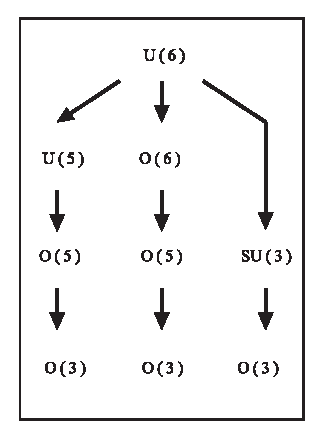
\includegraphics[scale=.65]{figure}
%
% If not, use
%\picplace{5cm}{2cm} % Give the correct figure height and width in cm
%
\caption{Please write your figure caption here}
\label{fig:A1}       % Give a unique label
\end{figure}

% For tables use
%
\begin{table}
\caption{Please write your table caption here}
\label{tab:A1}       % Give a unique label
%
% For LaTeX tables use
%
\begin{tabular}{p{2cm}p{2.4cm}p{2cm}p{4.9cm}}
\hline\noalign{\smallskip}
Classes & Subclass & Length & Action Mechanism  \\
\noalign{\smallskip}\hline\noalign{\smallskip}
Translation & mRNA$^a$  & 22 (19--25) & Translation repression, mRNA cleavage\\
Translation & mRNA cleavage & 21 & mRNA cleavage\\
Translation & mRNA  & 21--22 & mRNA cleavage\\
Translation & mRNA  & 24--26 & Histone and DNA Modification\\
\noalign{\smallskip}\hline\noalign{\smallskip}
\end{tabular}
$^a$ Table foot note (with superscript)
\end{table}
%

%%%%%%%%%%%%%%%%%%%%%%%% referenc.tex %%%%%%%%%%%%%%%%%%%%%%%%%%%%%%
% sample references
% %
% Use this file as a template for your own input.
%
%%%%%%%%%%%%%%%%%%%%%%%% Springer-Verlag %%%%%%%%%%%%%%%%%%%%%%%%%%
%
% BibTeX users please use
% \bibliographystyle{}
% \bibliography{}
%
\Extrachap{FURTHER READING}

\biblstarthook{}


\begin{thebibliography}{99.}%


\bibitem{ARTIN} ARTIN, E.: ``The Gamma Function,'' Holt, Rinehart and Winston, Inc., New York, 1964.
\bibitem{BOAS} BOAS, R. P.: ``A Primer of Real Functions,'' Carus Mathematical Monograph No. 13, John Wiley \& Sons, Inc., New York, 1960.
\bibitem{BUCKANALYSIS} BUCK, R. C. (ed.): ``Studies in Modern Analysis,'' Prentice-Hall, Inc., Englewood Cliffs, N.J., 1962.
\bibitem{BUCKCALCULUS} BUCK, R. C. (ed.): ``Advanced Calculus'' 2d ed., McGraw-Hill Book Company, New York, 1965.
\bibitem{BURKILL} BURKILL, J. C.: ``The Lebesgue Integral,'' Cambridge University Press, New York, 1951.
\bibitem{DIEUDONNE} DIEUDONNE, J.: ``Foundations of Modern Analysis,'' Academic Press, Inc., New York, 1960.
\bibitem{FLEMING} FLEMING, w. H.: ``Functions of Several Variables,'' Addison-Wesley Publishing Company, Inc., Reading, Mass., 1965.
\bibitem{GRAVES} GRAVES, L. M.: ``The Theory of Functions of Real Variables,'' 2d ed., McGraw-Hill Book Company, New York, 1956.
\bibitem{HALMOSMEASURE} HALMOS, P. R.: ``Measure Theory,'' D. Van Nostrand Company, Inc., Princeton, N.J., 1950.
\bibitem{HALMOSVECTOR} HALMOS, P. R.: ``Finite-dimensional Vector Spaces,'' 2d ed., D. Van Nostrand Company, Inc., Princeton, N.J., 1958.
\bibitem{HARDYPURE} HARDY, G. H.: ``Pure Mathematics,'' 9th ed., Cambridge University Press, New York, 1947.
\bibitem{HARDYFOURIER} HARDY, G. H. and ROGOSINSKI, W.: ``Fourier Series,'' 2d ed., Cambridge University Press, New York, 1950.
\bibitem{HERSTEIN} HERSTEIN, I. N.: ``Topics in Algebra,'' Blaisdell Publishing Company, New York, 1964.
\bibitem{HEWITT} HEWITT, E., and STROMBERG, K. : ``Real and Abstract Analysis,'' Springer Publishing Co., Inc., New York, 1965.
\bibitem{KELLOGG} KELLOGG, O. D.: ``Foundations of Potential Theory,'' Frederick Ungar Publishing Co., New York, 1940.
\bibitem{KNOPP} KNOPP, K.: ``Theory and Application of Infinite Series,'' Blackie \& Son, Ltd., Glasgow, 1928.
\bibitem{LANDAU} LANDAU, E. G. H.: ``Foundations of Analysis,'' Chelsea Publishing Company, New York, 1951.
\bibitem{MCSHANE} MCSHANE, E. J.: ``Integration,'' Princeton University Press, Princeton, N.J., 1944.
\bibitem{NIVEN} NIVEN, I. M.: ``Irrational Numbers,'' Carus Mathematical Monograph No. 11, John Wiley \& Sons, Inc., New York, 1956.
\bibitem{ROYDEN} ROYDEN, H. L.: ``Real Analysis,'' The Macmillan Company, New York, 1963.
\bibitem{RUDIN} RUDIN, W.: ``Real and Complex Analysis,'' 2d ed., McGraw-Hill Book Company, New York, 1974.
\bibitem{SIMMONS} SIMMONS, G. F.: ``Topology and Modern Analysis,'' McGraw-Hill Book Company, New York, 1963.
\bibitem{SINGER} SINGER, 1. M., and THORPE, J. A.: ``Lecture Notes on Elementary Topology and Geometry,'' Scott, Foresman and Company, Glenview, Ill., 1967.
\bibitem{SMITH} SMITH, K. T.: ``Primer of Modern Analysis'' Bogden and Quigley, Tarrytown-on-Hudson, N.Y., 1971.
\bibitem{SPIVAK} SPIVAK, M.: ``Calculus on Manifolds,'' W. A. Benjamin, Inc., New York, 1965.
\bibitem{THURSTON} THURSTON, H. A.: ``The Number System,'' Blackie \& Son, Ltd., London-Glasgow, 1956.




\end{thebibliography}

\backmatter%%%%%%%%%%%%%%%%%%%%%%%%%%%%%%%%%%%%%%%%%%%%%%%%%%%%%%%
%%%%%%%%%%%%%%%%%%%%%%acronym.tex%%%%%%%%%%%%%%%%%%%%%%%%%%%%%%%%%%%%%%%%%
% sample list of acronyms
%
% Use this file as a template for your own input.
%
%%%%%%%%%%%%%%%%%%%%%%%% Springer %%%%%%%%%%%%%%%%%%%%%%%%%%

\Extrachap{Acronyms and Abbreviations}
Here you can see a list of important acronyms.
\begin{description}[list]
\setlength{\labelwidth}{6em}
\item[ANSI]{\href{https://www.ansi.org/}{American National Standards Institute}}
\item[ASCII]{American Standard Code for Information Interchange}
\item[CPU]{Central Processing Unit}
\item[CUDA]{Compute Unified Device Architecture}
\item[DRAM]{Dynamic Random Access Memory}
\item[GNU]{GNU's Not Unix}
\item[GPU]{Graphics Processing Unit}
\item[grep]{g lobal(ly) search r egular e xpression p rint}
\item[NVRAM]{Non-Volatile Random Access Memory}
\item[pip]{Pip Installs Packages}
\item[RAM]{Random Access Memory}
\item[SDRAM]{Static Random Access Memory} 
\item[TPU]{Tensor Processing Unit}

\end{description}
%%%%%%%%%%%%%%%%%%%%%%acronym.tex%%%%%%%%%%%%%%%%%%%%%%%%%%%%%%%%%%%%%%%%%
% sample list of acronyms
%
% Use this file as a template for your own input.
%
%%%%%%%%%%%%%%%%%%%%%%%% Springer %%%%%%%%%%%%%%%%%%%%%%%%%%

\Extrachap{Glossary}


Use the template \emph{glossary.tex} together with the Springer document class SVMono (monograph-type books) or SVMult (edited books) to style your glossary\index{glossary} in the Springer layout.


\runinhead{GNU} GNU is not UNIX 

\runinhead{glossary term} Write here the description of the glossary term. Write here the description of the glossary term. Write here the description of the glossary term.

\runinhead{glossary term} Write here the description of the glossary term. Write here the description of the glossary term. Write here the description of the glossary term.

\runinhead{abs} datenwise

\runinhead{glossary term} Write here the description of the glossary term. Write here the description of the glossary term. Write here the description of the glossary term.


\Extrachap{Solutions}

\section*{Problems of Chapter~\ref{intro}}

\begin{sol}{prob1}
The solution\index{problems}\index{solutions} is revealed here.
\end{sol}


\begin{sol}{prob2}
\textbf{Problem Heading}\\
(a) The solution of first part is revealed here.\\
(b) The solution of second part is revealed here.
\end{sol}


\printindex

%%%%%%%%%%%%%%%%%%%%%%%%%%%%%%%%%%%%%%%%%%%%%%%%%%%%%%%%%%%%%%%%%%%%%%

\end{document}





